\documentclass[11pt]{article}

\usepackage[utf8]{inputenc}
\usepackage[T1]{fontenc}
\usepackage{lmodern}
\usepackage[margin=1in]{geometry}
\usepackage{amsmath,amssymb}
\usepackage{booktabs}
\usepackage{tabularx}
\usepackage{enumitem}
\usepackage{fvextra}
\usepackage{tikz}
\usetikzlibrary{shapes.geometric,arrows.meta,positioning}
\usepackage[numbers,sort&compress]{natbib}
\usepackage[hidelinks]{hyperref}

\newcommand{\code}[1]{\texttt{#1}}
\providecommand{\tightlist}{\setlength{\itemsep}{0pt}\setlength{\parskip}{0pt}}

\title{Proving Cognitive Theories in Lean:\\EPAM, Strategy Choice, and Their Combination}
\author{Jeff Shrager}
\date{Draft, \today}

\begin{document}
\maketitle

\begin{abstract}
We state cognitive theories as postulates in the Lean theorem prover and prove their phenomena as theorems that hold for every choice of the theories' parameters. CogLean is a library of general constructs and theory-neutral phenomena. EPAM (Feigenbaum and Simon) and the distributions-of-associations model of strategy choice (Siegler and Shrager, 1984) are its first two instances.

Combining the two theories in a model of 3-digit addition yields 18 predictions that neither makes alone, each proved by composing results already proved for the parts. The most distinctive is the \emph{confident error}: a fast, retrieved, wrong answer with no more backup use than on a familiar problem. Distributions of associations alone cannot produce it.

To check that the formal model says what its prose says, a fresh agent wrote a simulator from a prose specification alone, and we tested it against preregistered predictions and Lean's exact distributions. Every check whose hypothesis arose passed. The comparison also showed that five predictions are vacuous for the nets EPAM actually learns, exposed a gap in the formalization, and isolated an open choice on which the predicted learning sequence depends.
\end{abstract}

\section{Introduction}

What a cognitive theory predicts is usually established by running it. A simulation, with one set of parameters and stimuli, reproduces a published result. That shows the theory \emph{can} produce the result. It doesn't show which assumptions produced it, whether it survives a change of parameters, or whether a rival theory would produce it as well.

There are three kinds of evidence a theory can give:
\begin{enumerate}
  \item \textbf{One run} of one model: the theory can produce a behavior.
  \item \textbf{Every run} of one model, by exhaustive search or sampling: the behavior holds for that model, or how often.
  \item \textbf{Every model satisfying the postulates}: the postulates entail the behavior, under stated conditions.
\end{enumerate}

Most modelling evidence in psychology is of the first kind. This paper is about the third. We state theories as postulates in Lean~\cite{demoura2021}, a programming language that is also a proof assistant, and prove phenomena as theorems quantified over every encoding, net, strength, criterion and backup the postulates allow.

Proof brings three things a run does not:
\begin{itemize}
  \item \textbf{Which assumptions matter.} A proof uses some postulates and not others, and its hypotheses spell out the conditions it needs. A failed proof shows that a theory needs an assumption it never stated.
  \item \textbf{What is robust and what is accidental.} A theorem over all parameters settles whether a result comes from the theory or from a choice made in implementing it.
  \item \textbf{Possibility versus necessity.} Each theorem must say whether a behavior can occur, must occur, or occurs with a given probability.
\end{itemize}

The guarantee is relative. Lean checks that a theorem follows from the definitions. It doesn't check that the definitions capture the theory, still less that the theory is true of people. Section~\ref{sec:blind} addresses the first gap directly, with a blind simulation.

The contributions are:
\begin{enumerate}
  \item \textbf{A library, CogLean} (Section~\ref{sec:coglean}), in which constructs and theory-neutral phenomena are defined once and shared by theories.
  \item \textbf{Two theories as instances} (Section~\ref{sec:theories}): EPAM's discrimination nets and the distributions-of-associations (DOA) model of strategy choice, with their phenomena proved.
  \item \textbf{A combined theory} of 3-digit addition (Section~\ref{sec:multidigit}), whose 18 predictions are deduced, not simulated, by composing the two theories' results. One of them, the confident error, is a dissociation that DOA alone cannot produce.
  \item \textbf{A method for checking a formalization} (Section~\ref{sec:blind}): a simulator written blind from prose, preregistered predictions, and a comparison against Lean's exact distributions. It found no disagreement where the predictions applied, and three substantive problems where they didn't.
\end{enumerate}

\section{CogLean}
\label{sec:coglean}

CogLean is modelled on Mathlib~\cite{mathlib2020}: constructs are defined once, and every theory that uses them imports them. It has two parts:
\begin{itemize}
  \item \textbf{CogLib}, the general library. It imports no theory.
  \item \textbf{One package per theory}: EPAM, StrategyChoice, and MultiDigit. MultiDigit requires the other two.
\end{itemize}

\begin{table}[h]
\centering
\begin{tabularx}{\linewidth}{@{}lX@{}}
\toprule
Layer & Contents in CogLib \\
\midrule
Representations & feature codes (lists of bits); finite distributions with exact rational probabilities \\
Memory structures & discrimination nets; cues \\
Processes & discrimination learning; association; sampled retrieval with a confidence criterion and a search length \\
Control & noticing orders: the order in which features are scanned for a difference \\
Phenomena & theory-neutral statements: learning to criterion, stimulus generalization, oscillation, retroactive interference, the serial position effect \\
\bottomrule
\end{tabularx}
\caption{The layers of CogLib.}
\end{table}

A theory's package holds:
\begin{itemize}
  \item its postulates, each stated as a choice of CogLib constructs and cited to its source, with simplifications listed;
  \item its parameters;
  \item its experiments, computed by the Lean kernel;
  \item its phenomena, proved.
\end{itemize}

A phenomenon is stated once, independently of any mechanism, as a property a learner may have. A theory then proves that its learners have it, or that they lack it.

Shared definitions make theories comparable. For example, ``any learner whose learning does not interfere reaches criterion'' is proved once in CogLib. Discrimination nets are proved not to interfere, also in CogLib. EPAM then gets learning to criterion in one line, and so will any later theory whose learning does not interfere. Two theories explain a phenomenon in the same way when their proofs go through the same lemma.

Three engineering choices keep the library light and the proofs trustworthy:
\begin{itemize}
  \item \textbf{Core Lean only, no Mathlib.} The whole library builds in seconds.
  \item \textbf{Exact probabilities.} They are core rationals, so concrete distributions are computed exactly by the kernel (\code{decide +kernel}).
  \item \textbf{Fully proved.} There is no \code{sorry}, and \code{\#print axioms} shows only Lean's standard axioms (\code{propext}, \code{Quot.sound}, \code{Classical.choice}).
\end{itemize}

\section{Two theories}
\label{sec:theories}

\subsection{EPAM: recognition by discrimination net}

EPAM~\cite{feigenbaum1959,feigenbaum1962} recognizes a stimulus by sorting its code, a vector of bits, down a discrimination net. Each test examines one feature; each terminal holds an image or nothing. A stimulus confused with a stored one is learned by growing a test, at that terminal, on the first feature in the noticing order where the two differ. We formalize the propositions of P-1817, not the IPL-V program.

The mechanism-level results are proved once in CogLib, for any net, code and noticing order:
\begin{itemize}
  \item what a stimulus is recognized as depends only on the features examined on its path;
  \item learning makes the new stimulus recognized, and never disturbs another's recognition;
  \item if each image is stored once, a stimulus confused with a stored image agrees with it on every feature its path examines;
  \item every net learned from an empty one stores each image once and recognizes each as itself.
\end{itemize}

From these, EPAM's phenomena follow through CogLib's theory-neutral statements. The \textbf{necessary} ones are learning to criterion, stimulus generalization and the bowed serial position curve. The \textbf{possible} ones are oscillation and retroactive inhibition. A full serial-anticipation experiment (Fig.~4.1 of P-1817) is computed by the kernel and compared, response by response, with the published one.

\subsection{Strategy choice: distributions of associations}

In the distributions-of-associations model~\cite{siegler1984}, a child adding single digits has associations of varying strength between the problem and possible answers.
\begin{enumerate}
  \item On each trial the child sets a confidence criterion $c$ and a search length $n$.
  \item A search draws an answer in proportion to its strength, and states it if the strength exceeds $c$, for up to $n$ searches.
  \item If retrieval is exhausted, the child puts up fingers, which adds strength to the correct answer, and searches once more.
  \item Failing that, the child counts the fingers, with fixed chances of skipping or double-counting.
  \item Every stated answer is strengthened, a correct one twice as much.
\end{enumerate}

Write $R$ for the chance that one search clears the criterion. Retrieval is exhausted with probability $(1-R)^n$, and states an answer with property $P$ with probability $Q_P \cdot G_n$, where
\[
  G_n = 1 + (1-R) + \cdots + (1-R)^{n-1}.
\]
Five of the twelve theorems predict dissociations that can be tested:
\begin{itemize}
  \item \textbf{Persistence and accuracy dissociate.} Search length changes how often children retrieve, not how accurately.
  \item \textbf{Retrieval doesn't depend on the backups.} Retrieval is unchanged however good or available the backup strategies are. A test of this is a test of the chapter's central claim, that strategy choice needs no metacognitive governor.
  \item \textbf{Counting errors don't depend on the associations.} This is the chapter's ``nonintuitive prediction'', proved exactly.
  \item \textbf{Strengthening the correct answer never raises retrieval errors}, at any criterion or search length.
  \item \textbf{Strengthening the correct answer can raise overt strategy use}, when a strong wrong competitor falls below the criterion.
\end{itemize}

\section{Combining theories: multi-digit addition}
\label{sec:multidigit}

The combined model nests DOA's architecture one level up. A child adding two 3-digit numbers may simply know the answer to a familiar problem such as $100+100$, or may work it out column by column. When the net hasn't learned to tell two problems apart, it confuses them, and retrieval runs on the wrong problem's associations.

\subsection{Postulates}

\begin{description}[leftmargin=1.5em]
  \item[M1, problem code.] A problem is coded as features, including features for each digit of each addend. Agreeing on all of a digit's features means having the same digit.
  \item[M2, recognition.] An EPAM net stores the codes of familiar problems, and a problem's code is sorted down it.
  \item[M3, whole-problem retrieval.] If the problem is recognized as the stored problem $q$, DOA retrieval runs on $q$'s associations.
  \item[M4, column backup.] If nothing is recognized, or retrieval is exhausted, each column is added by a single-digit DOA trial, units first, carrying the tens of each result.
  \item[M5, learning.] EPAM discrimination after a confusion, and DOA strengthening of stated answers.
  \item[M1a--M1c, further features,] as laws an encoding may satisfy: zero flags, digit magnitudes as nine thresholds, and an unordered fact per column.
\end{description}

\begin{figure}[t]
\centering
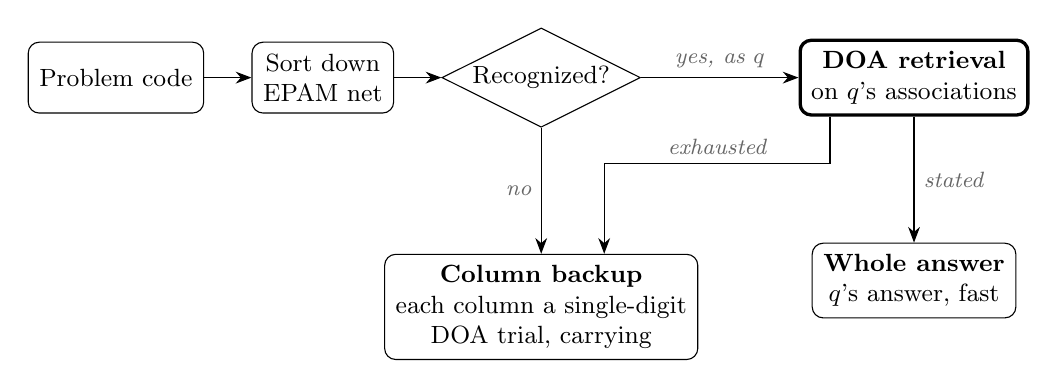
\begin{tikzpicture}[
  font=\small,
  box/.style={draw, rounded corners, minimum height=9mm, align=center, inner sep=4pt},
  dec/.style={draw, diamond, aspect=2, inner sep=1pt, align=center},
  arr/.style={-{Stealth[length=2mm]}},
  lab/.style={font=\footnotesize\itshape, text=black!60}
]
  \node[box] (code) {Problem code};
  \node[box, right=6mm of code] (net) {Sort down\\EPAM net};
  \node[dec, right=6mm of net] (rec) {Recognized?};
  \node[box, right=20mm of rec, very thick] (ret) {\textbf{DOA retrieval}\\on $q$'s associations};
  \node[box, below=16mm of rec] (cols) {\textbf{Column backup}\\each column a single-digit\\DOA trial, carrying};
  \node[box, below=16mm of ret] (whole) {\textbf{Whole answer}\\$q$'s answer, fast};
  \draw[arr] (code) -- (net);
  \draw[arr] (net) -- (rec);
  \draw[arr] (rec) -- node[lab, above] {yes, as $q$} (ret);
  \draw[arr] (rec) -- node[lab, left] {no} (cols);
  \draw[arr] (ret) -- node[lab, right] {stated} (whole);
  \draw[arr] (ret.south west) ++(4mm,0) |- ++(0,-6mm) -| node[lab, pos=0.25, above] {exhausted} ([xshift=8mm]cols.north);
\end{tikzpicture}
\caption{A trial on a 3-digit problem (M1--M4). Recognition decides whose associations are searched; only failed recognition or exhausted retrieval sends the problem to the columns. When $x$ is confused with $q$, $x$ gets $q$'s answer at $q$'s low rate of column use: a confident error (Prediction~4).}
\label{fig:trial}
\end{figure}

Every postulate is a parameter. There is no table of associations for a million problems. Each prediction holds for every encoding, net, set of strengths, criterion, search length and backup that satisfy the postulates. Figure~\ref{fig:trial} shows a trial.

\subsection{Predictions}

Write $R_q$ for the chance that one search of $q$'s associations clears the criterion, and call $q$'s associations \textbf{sharp} if no answer but $q$'s sum clears it. Only three new lemmas were needed:
\begin{itemize}
  \item \textbf{Lemma A:} a confusion is with a code that looks the same along the path.
  \item \textbf{Lemma B:} every net EPAM learns satisfies Lemma A's hypothesis.
  \item \textbf{Lemma C:} a confusion keeps every property that the features on its path determine.
\end{itemize}

\begin{table}[t]
\centering
\small
\begin{tabularx}{\linewidth}{@{}rXl@{}}
\toprule
\# & Prediction & Rests on \\
\midrule
1 & Columns are used with probability 1 if the problem is not recognized, and $(1-R_q)^n$ if it is recognized as $q$ & DOA Thm 1 \\
2 & Whole-problem retrieval on $x$ is exactly retrieval on what $x$ is recognized as & DOA Thm 2 \\
3 & A problem confused with a sharp $q$ gets $q$'s sum on every whole-problem trial & 2 \\
4 & \textbf{Confident errors:} if $x$ (with a different sum) is confused with a sharp $q$, every whole-problem answer on $x$ is wrong, yet $x$ falls back on the columns exactly as rarely as $q$ does & 1, 3 \\
5 & A confusion with a problem of the same sum, such as the commuted problem, is harmless & 2 \\
6 & If the path tests the hundreds digits, a confused answer is within 200; with the tens too, within 20 & Lemmas A, B \\
7 & Learning other problems never changes how a studied problem is answered & EPAM \\
8 & Problems that agree on the first $k$ noticed features cost at least $k$ scanning steps & EPAM \\
9 & With correct carrying, the column answer is $r_0 + 10r_1 + 100r_2$: carrying adds no error & arithmetic \\
10 & A column error is a single-digit DOA error moved to its place: off by exactly $10^j\delta$ & 9 \\
11 & Discrimination removes a confusion, and only that one, and keeps the net clean & Lemma B, 7 \\
12 & A newly discriminated problem whose associations don't yet clear the criterion is worked out by the columns & 1 \\
13 & If the path tests a digit's zero flag, a confusion keeps whether that digit is 0 & Lemma C \\
14 & A problem confused with a round one is that problem, once the zeros of tens and units and the hundreds digits are tested & 6, 13 \\
15 & A confused digit lies between the same tested thresholds as the true one & Lemma C \\
16 & Two digits differ on exactly $|d-e|$ of the nine thresholds, so close digits are the ones confused & 8 \\
17 & With every column's fact tested, a confusion has the right sum & Lemma C, 5 \\
18 & With the tens and units facts tested, a confusion's error is a multiple of 100 (with units alone, of 10) & Lemma C \\
\bottomrule
\end{tabularx}
\caption{The predictions of the combined model, each a Lean theorem.}
\label{tab:predictions}
\end{table}

Table~\ref{tab:predictions} lists the predictions. Prediction~4 is the one neither theory makes alone. In DOA, a problem's retrieval errors and its backup use come from the same distribution: a flat distribution raises both. Confusion gives a problem another problem's distribution, with that problem's low backup use and all of its errors.

Together, Predictions 4, 11 and 12 predict a learning sequence that can be looked for:
\begin{enumerate}
  \item a fast, confident error;
  \item after feedback and discrimination, slow column work;
  \item as correct answers are strengthened, fluent and correct retrieval.
\end{enumerate}

\subsection{Worked cases}

The worked cases are computed by the kernel. They are checks that the theorems apply, not evidence.
\begin{itemize}
  \item \textbf{Binary-coded digits.} A net that has learned $100+100$ and $100+200$ tests a single bit, and takes $150+100$ for $100+100$. With search length 1, it answers 200 with probability $45/46$.
  \item \textbf{Zero flags.} Under a 360-feature encoding, a net learned from $100+100$ and $120+100$ tests the first addend's tens zero flag. It takes $150+100$ for $120+100$, never for the round $100+100$.
  \item \textbf{Thresholds.} A net learned from $700+100$ and $800+100$ takes $600+100$ for its neighbour $700+100$. The binary-coded net takes it for $800+100$, because $7 = 0111$ and $8 = 1000$ share no bit.
\end{itemize}

\section{Checking the formalization by blind simulation}
\label{sec:blind}

Lean guarantees that the theorems follow from the definitions, not that the definitions say what the prose model says. We tested that link with a second implementation, built so that it could not simply copy the first.

\subsection{Method}

\begin{enumerate}
  \item \textbf{Specification.} We wrote the model as a 10\,KB prose specification (Appendix~\ref{app:spec}), with no Lean names, theorems or predictions. Points the prose leaves open are listed as open choices for the implementer to settle and document:
  \begin{itemize}
    \item O1: how correctness is judged when strengthening after a confusion;
    \item O2: the initial associations of a newly discriminated problem;
    \item O3: whether column answers strengthen whole-problem associations.
  \end{itemize}
  \item \textbf{Preregistration.} Before the simulator existed, we committed a list of checks. Each check names a theorem, the observable statistic, its hypothesis as read from the log, and the tolerance:
  \begin{itemize}
    \item exact relations: zero violations allowed;
    \item probabilities: a frequency within $4\sigma$ of the predicted value, or exactly 0 or $N$ when the predicted probability is 0 or 1.
  \end{itemize}
  A check whose hypothesis never arose is reported as vacuous, not as passed.
  \item \textbf{Blind implementation.} A fresh agent (a Claude model) received the specification and nothing else. It worked in an empty directory, and an audit of its tool calls showed that it read only files it had written. Its simulator is committed unmodified.
  \item \textbf{Exact export.} Lean evaluates the model's exact trial distributions, as rationals, on four instances, including the worked cases above.
  \item \textbf{Comparison.} A harness generated 30 random fixed-mode instances and 20 random learning-mode instances, and ran the checks. The instances varied the encoding, the noticing order, the familiar sets, the strengths, the criteria and the search lengths.
\end{enumerate}

\subsection{Results}

Every check whose hypothesis arose passed, with no failures (Table~\ref{tab:results}).

\begin{table}[h]
\centering
\begin{tabularx}{\linewidth}{@{}Xr@{}}
\toprule
Check & Tests \\
\midrule
Lean exact distributions, 4 instances & 243 \\
Strategy nesting, retrieval by route, confident errors (Predictions 1--4), with Lemma A & 14{,}320 \\
Same-sum confusions (Prediction 5) & 11 \\
Carrying and column errors (Predictions 9 and 10) & 287{,}799 \\
Zeros and thresholds (Predictions 13 and 15) & 67 \\
Learning: non-interference, discrimination, then columns (Predictions 7, 11, 12) & 165{,}861 \\
Near misses, round problems, column facts (Predictions 6, 14, 17, 18) & vacuous \\
\bottomrule
\end{tabularx}
\caption{Checks of the blind simulator, with no failures.}
\label{tab:results}
\end{table}

The prose specification and the Lean formalization therefore agree on recognition, EPAM learning, DOA retrieval, the backup strategies and carrying. The comparison also produced three findings.

\paragraph{Five predictions say little about learned nets.} Predictions 6, 14, 17 and 18 require the path to test every feature of a digit or a column. That is 4 bits, 9 thresholds or 100 fact features. EPAM grows one test per confusion, so in no learned net did a path ever meet these hypotheses. The theorems are true but nearly vacuous for the nets EPAM learns. They need versions about the features that are tested. For example: the tested bits of a digit restrict it to a set, which bounds the error.

\paragraph{Zero total strength is a gap in the formalization.} In Lean, sampling from associations with total strength 0 divides by 0, and the trial then has probability mass 0. The theorems avoid the case by assuming the total is nonzero. The simulator reads it as retrieval exhausted, which is the natural reading of the model. This matters, because it is what makes the most natural choice for O2 work.

\paragraph{The learning sequence depends on an open choice.} The sequence of Section~\ref{sec:multidigit} appeared in 40 of 48 problems when a newly discriminated problem starts with no associations. With only the correct answer, the column phase was skipped. When the new problem copied its neighbour's associations, the confusion's error was stated, strengthened and stated again. 7 of 44 problems stayed trapped, and 35 were still mixed at the end. The blind implementer predicted this trap from the specification alone. Which choice is right is a question about the theory, not about the code.

The implementer's other readings matched Lean's: for example, single-digit associations belong to ordered pairs.

\section{Related work}

Formal methods have been applied to psychological theories before. What is new here is the combination: a general-purpose proof assistant, theorems quantified over whole classes of models, phenomena as the targets of proof, and one cumulative library in which theories share definitions.

\begin{table}[h]
\centering
\small
\begin{tabularx}{\linewidth}{@{}p{0.3\linewidth}p{0.22\linewidth}X@{}}
\toprule
Approach & Formalism & What is established \\
\midrule
Theory representation by logic programming~\cite{rohner2021} & Prolog & conclusions entailed by a verbal theory's premises, with their derivations. Closest in aim; CogLean adds machine-checked proofs over unbounded classes of models \\
Automata-based formalization of verbal theories~\cite{finkel2025} & communicating automata & an analyzable model of a theory stated in words \\
Formal semantics of ACT-R~\cite{gall2017semantics,gall2017confluence} & operational semantics, Constraint Handling Rules & theorems about an architecture (such as confluence), not about phenomena \\
Model checking ACT-R models~\cite{langenfeld2019} & timed automata & properties of every execution of one model \\
Verification in a common model of cognition~\cite{laird2017,ganeriwala2025} & state machines, nuXmv & correctness and termination of small ACT-R and Soar models \\
Executable cognitive models (ACT-R, Soar, EPAM) & simulation programs & that a fitted model reproduces observed data \\
\bottomrule
\end{tabularx}
\caption{Formal approaches to psychological theory.}
\end{table}

The Common Model of Cognition~\cite{laird2017} is the nearest relative in scale. It looks for the architectural commitments that many theories share. CogLean pursues the same convergence at the level of definitions and theorems: a shared commitment is a shared module, and a shared explanation is a shared lemma.

The blind simulation borrows from N-version programming~\cite{avizienis1985}, where independent teams implement one specification so that their disagreements reveal faults, and from preregistration in empirical science. We are not aware of either being used to check a formalized cognitive theory.

\section{Discussion}

\paragraph{What proof bought.} The multi-digit predictions came from composing results already proved for the parts. Only three new lemmas about nets were needed. The proofs also say what each prediction rests on. For example, confident errors need the criterion and search length not to depend on the route. A failed test of Prediction~4 would therefore point at a specific assumption, not at the model as a whole.

\paragraph{What simulation bought.} A proof can be true and still say little. Nothing in Lean flagged that the near-miss and column-fact theorems need hypotheses that learned nets never meet. The simulation found it by counting how often each hypothesis arose. The same goes for the zero-strength case: it lies outside every theorem, and in the simulator it is the natural default. Proof and simulation are complementary in a way the slogan ``simulation explores, proof settles'' understates. Simulation also checks what proof is about.

\paragraph{Open choices are theory.} The specification's open choices were written as implementation details. One of them turned out to decide whether the model's central learning prediction holds. A formalization that is silent on a point is silent in a way a simulation can't be: running the model forces a choice. The blind implementer, writing from prose, both made the choice and flagged what turns on it.

\paragraph{Limitations.}
\begin{itemize}
  \item The theorems are qualitative or exact-probability results about the postulates. None is fitted to data, and none is yet tested against children's 3-digit addition.
  \item The blind implementer was a language model. Its blindness rests on an instruction and on the audit of its tool calls, not on anything that enforces it.
  \item The criterion and search length are fixed per trial, and the columns are added independently, with error-free carrying.
\end{itemize}

\paragraph{Next steps.}
\begin{enumerate}
  \item Restate the vacuous predictions in terms of the features that are tested.
  \item Define retrieval with zero total strength as exhausted.
  \item Settle O2, and prove the learning sequence over many trials.
  \item State ACT-R's declarative memory as a rival theory of the same single-digit data. ACT-R's tutorial model fits the 4-year-olds' answer distributions by partial matching, with no backup strategy, criterion or learning. The two theories can then be compared on the same theory-neutral statements, theorem by theorem. Strategy discovery (SCADS~\cite{shrager1998}) is a further candidate.
\end{enumerate}

\paragraph{Code.} \url{https://github.com/jeffshrager/CogLean}

\bibliographystyle{unsrtnat}
\bibliography{refs}

\appendix
\section{The prose specification}
\label{app:spec}

This is the specification given to the blind implementer (Section~\ref{sec:blind}), verbatim except for layout: its sections 1--10 are numbered A.1--A.10 here, and references in it to ``section $N$'' mean A.$N$.

{\small\sloppy
This document specifies a model of how a child adds two 3-digit numbers. Implement it as a stochastic simulation in Python. It is self-contained: everything you need is here, and where the model leaves something open, that is said explicitly (section 8).

\subsection{Problems}\label{problems}

A problem is a + b, with whole numbers 0 $\le$ a, b $\le$ 999. Its correct answer is a + b.

\begin{itemize}
\tightlist
\item
  Each addend has three digits: hundreds, tens and units. A number below 100 has hundreds digit 0, and so on.
\item
  A \textbf{column} is a place (hundreds, tens or units) together with the two digits of the addends in that place.
\item
  Write problems as strings \texttt{"a+b"}, e.g.~\texttt{"150+100"}.
\end{itemize}

\subsection{Codes}\label{codes}

A problem reaches the child as a \textbf{code}: a vector of bits, called features, indexed from 0. A feature beyond the end of a code reads as 0. There are two encodings. Addends are numbered first = 0 and second = 1; places are numbered hundreds = 0, tens = 1 and units = 2.

\subsubsection{\texorpdfstring{\texttt{bcd} (24 features)}{bcd (24 features)}}\label{bcd-24-features}

\begin{itemize}
\tightlist
\item
  Feature \texttt{addend*12\ +\ place*4\ +\ k}, for k = 0..3, is bit k of that digit in binary. Bit 0 is the least significant.
\item
  Example: the digit 6 = 0110 has bit 0 = 0, bit 1 = 1, bit 2 = 1 and bit 3 = 0.
\end{itemize}

\subsubsection{\texorpdfstring{\texttt{rich} (360 features)}{rich (360 features)}}\label{rich-360-features}

\begin{itemize}
\tightlist
\item
  \textbf{Digit blocks.} For each digit, a block of 10 features starting at \texttt{(addend*3\ +\ place)*10}:

  \begin{itemize}
  \tightlist
  \item
    offset 0: 1 if the digit is 0 (the \textbf{zero flag});
  \item
    offset 1 + k, for k = 0..8: 1 if the digit is greater than k (a \textbf{threshold}).
  \end{itemize}
\item
  \textbf{Column facts.} For each place, 100 features starting at \texttt{60\ +\ place*100}. Exactly one is 1: the one at offset \texttt{min*10\ +\ max}, where min and max are the smaller and the larger of the column's two digits. So 3+4 and 4+3 in a column set the same feature.
\end{itemize}

\subsubsection{Noticing orders}\label{noticing-orders}

A \textbf{noticing order} is a list of feature indices: the order in which features are scanned for a difference (section 3). The parameter file gives it as an explicit list, or as one of these names:

\begin{itemize}
\tightlist
\item
  \texttt{bcd\_hundreds\_first}. For place = hundreds, tens, units (in that order); then addend = first, second; then k = 0..3: the bcd feature for (addend, place, k).
\item
  \texttt{rich\_default}, the concatenation of three lists:

  \begin{enumerate}
  \def\labelenumi{\arabic{enumi}.}
  \tightlist
  \item
    The zero flags. For place = hundreds, tens, units; then addend = first, second.
  \item
    The thresholds. For place = hundreds, tens, units; then addend = first, second; then k = 0..8.
  \item
    The column facts. For place = hundreds, tens, units; then offset 0..99.
  \end{enumerate}
\end{itemize}

\subsection{Recognition: a discrimination net}\label{recognition-a-discrimination-net}

The child's memory of familiar problems is a \textbf{discrimination net} (EPAM). It is a binary tree:

\begin{itemize}
\tightlist
\item
  A \textbf{terminal} holds an image (a stored code) or nothing.
\item
  A \textbf{test} names one feature and has two branches, one for 0 and one for 1.
\end{itemize}

\textbf{Recognition} sorts a code down the net: at each test, take the branch given by the code's value on that feature. The result is the image at the terminal reached, which may be nothing. The \textbf{path} is the list of features tested on the way down. The problem is \textbf{recognized as} the problem whose code that image is. Images are always codes of problems, so keep track of which problem each image came from.

\textbf{Learning a code x} into the net:

\begin{enumerate}
\def\labelenumi{\arabic{enumi}.}
\tightlist
\item
  Sort x down the net to a terminal.
\item
  If the terminal holds nothing, put x there.
\item
  If it holds x itself, do nothing.
\item
  If it holds a different image z, scan the noticing order for the first feature f on which x and z differ.

  \begin{itemize}
  \tightlist
  \item
    If there is one, replace the terminal by a test on f, whose two branches are terminals holding x and z, each on the side of its own value of f.
  \item
    If no feature in the order differs, do nothing.
  \end{itemize}
\end{enumerate}

Nothing else in the net changes. The net starts empty (one terminal holding nothing). The \textbf{familiar problems} in the parameter file are learned into it in the order given.

\subsection{Retrieval from a distribution of associations}\label{retrieval-from-a-distribution-of-associations}

Retrieval works on \textbf{associations}: a finite list of possible answers, each with a strength $\ge$ 0, with total strength T \textgreater{} 0. It also uses a \textbf{confidence criterion} c and a \textbf{search length} n.

\begin{itemize}
\tightlist
\item
  \textbf{A search} draws one answer, each with probability strength/T.
\item
  If the drawn answer's strength is strictly greater than c, it is \textbf{stated}, and retrieval ends.
\item
  Otherwise search again, up to n searches in all.
\item
  If no answer is stated after n searches, retrieval is \textbf{exhausted}.
\end{itemize}

\subsection{Single-digit addition (used in each column)}\label{single-digit-addition-used-in-each-column}

Adding two digits d + e uses the associations of the single-digit problem d + e (its answer list and strengths), a criterion c1 and a search length n1. It proceeds in three stages; the \textbf{strategy} is the one that produces the answer.

\begin{enumerate}
\def\labelenumi{\arabic{enumi}.}
\tightlist
\item
  \textbf{Retrieval}: as in section 4. If an answer is stated, that is the answer.
\item
  \textbf{Fingers}: if retrieval is exhausted, the child puts up d + e fingers.

  \begin{itemize}
  \tightlist
  \item
    Add strength \texttt{elab} to the answer d + e.
  \item
    Then divide every strength (including that one) by 1 + \texttt{elab}.
  \item
    Make exactly one search with these new strengths. If the drawn answer's new strength exceeds c1, state it.
  \item
    These new strengths are used for this one search only; nothing is changed permanently.
  \end{itemize}
\item
  \textbf{Counting}: otherwise the child counts the d + e fingers.

  \begin{itemize}
  \tightlist
  \item
    Each of the d + e objects is skipped with probability \texttt{qs}, counted twice with probability \texttt{qd}, and counted once otherwise, independently.
  \item
    The answer is the total count.
  \end{itemize}
\end{enumerate}

\subsection{A trial on a 3-digit problem x}\label{a-trial-on-a-3-digit-problem-x}

\begin{enumerate}
\def\labelenumi{\arabic{enumi}.}
\tightlist
\item
  Recognize x's code in the net.
\item
  If x is recognized as a stored problem y, retrieve (section 4) using \textbf{y's} whole-problem associations, with criterion c and search length n.~If an answer is stated, that is the trial's answer, by the \textbf{whole} route.
\item
  If nothing is recognized, or retrieval is exhausted, work x out by the \textbf{columns} route:

  \begin{itemize}
  \tightlist
  \item
    Add the units column's digits (section 5); call the result r0. Write r0 mod 10, and carry $\lfloor$r0 / 10$\rfloor$.
  \item
    Add the tens column's digits; call the result r1. Add the carry: s1 = r1 + $\lfloor$r0 / 10$\rfloor$. Write s1 mod 10, and carry $\lfloor$s1 / 10$\rfloor$.
  \item
    Add the hundreds column's digits; call the result r2. Write r2 + $\lfloor$s1 / 10$\rfloor$ as the hundreds (it may exceed 9).
  \item
    The answer is the number written. Note that column results can exceed 18 through counting errors; the carry rule handles any size.
  \end{itemize}
\end{enumerate}

Each column uses its own single-digit problem's associations, and the three columns are added independently.

\subsection{Learning (between trials)}\label{learning-between-trials}

When learning is on, after each trial:

\begin{enumerate}
\def\labelenumi{\arabic{enumi}.}
\tightlist
\item
  \textbf{Strengthening (single-digit).} For each column added in the trial, the stated single-digit answer's strength in that single-digit problem's associations increases by \texttt{inc1}, or by \texttt{2*inc1} if that answer is correct for the column (d + e). This happens whichever strategy produced it. If the answer isn't yet in the answer list, add it with strength 0 first.
\item
  \textbf{Strengthening (whole problem).} If the answer came by the whole route, the stated answer's strength in the associations that were used increases by \texttt{inc}, or \texttt{2*inc} if it is correct. ``Correct'' here is subject to open choice O1.
\item
  \textbf{Discrimination.} If the answer came by the whole route and was wrong (feedback tells the child), learn x's code into the net (section 3), with new associations for x (open choice O2).
\item
  \textbf{Column answers and whole associations} (open choice O3).
\end{enumerate}

\subsection{Open choices}\label{open-choices}

The model doesn't settle these. Choose a default, document it in \texttt{IMPLEMENTATION\_NOTES.md}, and expose each as a parameter.

\begin{itemize}
\tightlist
\item
  \textbf{O1.} In whole-route strengthening, is ``correct'' judged against the true sum of x, or against the sum of the problem y whose associations were used?
\item
  \textbf{O2.} What are the initial associations of a newly discriminated problem: its answer list, its strengths?
\item
  \textbf{O3.} Does a columns-route answer change the whole-problem associations of x? If so, how, and only when x is stored in the net?
\item
  \textbf{O4.} Anything else you find underdetermined. List it.
\end{itemize}

\subsection{Interface}\label{interface}

\subsubsection{Program}\label{program}

Write \texttt{mdsim.py}: Python 3, standard library only, with \texttt{fractions.Fraction} for all strengths and probabilities. Floating point may be used only to compare against random draws.

\begin{itemize}
\tightlist
\item
  Command line: \texttt{python3\ mdsim.py\ PARAMS.json\ -\/-out\ LOG.jsonl}
\item
  Library: \texttt{simulate(params:\ dict)\ -\textgreater{}\ Iterator{[}dict{]}}, which yields the same records.
\item
  Use \texttt{random.Random(seed)} for all randomness.
\end{itemize}

\subsubsection{Parameter file (JSON)}\label{parameter-file-json}

Fractions are strings such as \texttt{"9/10"}, or numbers.

\begin{Verbatim}[breaklines,breakanywhere,fontsize=\footnotesize]
{
  "encoding": "bcd" | "rich",
  "order": "bcd_hundreds_first" | "rich_default" | [feature indices],
  "familiar": ["100+100", "100+200"],
  "answers": [200, 250, 300],
  "whole": {"100+100": {"200": "9/10", "250": "1/100", "300": "1/100"}, "...": {}},
  "c": "1/2",
  "n": 1,
  "single": {"answers": [0, 1, ..., 18], "default": {"correct": "1/2", "other": "1/50"},
             "overrides": {"2+3": {"4": "3/10", "5": "1/2"}}},
  "c1": "1/2",
  "n1": 1,
  "elab": "1/20",
  "qs": "1/20",
  "qd": "1/20",
  "learning": false,
  "inc": "1/20",
  "inc1": "1/20",
  "open_choices": {"O1": "...", "O2": "...", "O3": "..."},
  "schedule": ["150+100", "100+100"],
  "repeats": 1000,
  "seed": 1
}
\end{Verbatim}

\begin{itemize}
\tightlist
\item
  \textbf{\texttt{whole}}: the whole-problem associations of each familiar problem, over \texttt{answers}. An answer missing from a problem's table has strength 0.
\item
  \textbf{\texttt{single}}: associations for every d + e (d, e = 0..9).

  \begin{itemize}
  \tightlist
  \item
    Over \texttt{answers}, the correct answer d + e has strength \texttt{default.correct} and every other answer \texttt{default.other}.
  \item
    \texttt{overrides} replaces the given entries for a given single-digit problem.
  \end{itemize}
\item
  \textbf{\texttt{schedule}}: the run is \texttt{repeats} passes through the schedule, one trial per problem per pass, in order.

  \begin{itemize}
  \tightlist
  \item
    With learning off, the net and all strengths stay fixed throughout.
  \item
    With learning on, they change as in section 7.
  \end{itemize}
\end{itemize}

\subsubsection{Log (JSON lines, one record per trial)}\label{log-json-lines-one-record-per-trial}

\begin{Verbatim}[breaklines,breakanywhere,fontsize=\footnotesize]
{"trial": 0, "pass": 0, "problem": "150+100",
 "recognized_as": "100+100" | null, "path": [features tested],
 "route": "whole" | "columns",
 "searches": number of whole-route searches made,
 "columns": [{"place": "units", "digits": [0, 0], "strategy": "retrieval" | "fingers" | "counting", "answer": 0}, ...] | [],
 "answer": 200, "correct": false,
 "net_learned": true | false}
\end{Verbatim}

\begin{itemize}
\tightlist
\item
  \texttt{columns} lists the units, tens and hundreds entries when the columns route is used, and is empty otherwise.
\item
  \texttt{net\_learned} says whether discrimination changed the net after this trial.
\end{itemize}

\subsection{Deliverables}\label{deliverables}

\begin{itemize}
\tightlist
\item
  \texttt{mdsim.py}.
\item
  \texttt{IMPLEMENTATION\_NOTES.md}: your choices for O1--O4, anything you found ambiguous, and a list of every file you read while working.
\item
  A smoke test: \texttt{python3\ mdsim.py\ example.json\ -\/-out\ /dev/stdout\ \textbar{}\ head}, with an \texttt{example.json} of your own.
\end{itemize}

}

\end{document}
